\titledquestion{Multiple Choices}

Each question has \textbf{one or more} correct answer(s). Select all the correct answer(s). For each question, you will get 0 points if you select one or more wrong answers, but you will get 1 point if you select a non-empty subset of the correct answers.

Write your answers in the following table.

%%%%%%%%%%%%%%%%%%%%%%%%%%%%%%%%%%%%%%%%%%%%%%%%%%%%%%%%%%%%%%%%%%%%%%%%%%%
% Note: The `LaTeX' way to answer a multiple-choice question is to replace `\choice'
% with `\CorrectChoice', as what you did in the first question. However, there are still
% many students who would like to handwrite their homework. To make TA's work easier,
% you have to fill in your selected choices in the table below, no matter whether you use 
% LaTeX or not.
%%%%%%%%%%%%%%%%%%%%%%%%%%%%%%%%%%%%%%%%%%%%%%%%%%%%%%%%%%%%%%%%%%%%%%%%%%%

\begin{table}[htbp]
	\centering
	\begin{tabular}{|p{2cm}|p{2cm}|p{2cm}|p{2cm}|p{2cm}|}
		\hline 
		(a) & (b) & (c) & (d)  \\
		\hline
  		%%%%%%%%%%%%%%%%%%%%%%%%%%%%%%%%%%%%%%%%%%%%%%%%%%%%%%%%%%
		% YOUR ANSWER HERE.
		   &  &  &  \\
            %%%%%%%%%%%%%%%%%%%%%%%%%%%%%%%%%%%%%%%%%%%%%%%%%%%%%%%%%%
		\hline
	\end{tabular} 
\end{table}

\begin{parts}


\part[2] Which of the following statements about topological sort is/are true?
\begin{choices}
    \choice A sub-graph of a DAG may not have a topological sorting.
    \choice Any directed tree has a topological sorting.
    \choice It's possible for a DAG to have multiple topological sortings.
    \choice Since we have to scan all vertices to find those with zero in-degree in each iteration, the run time of topological sort is $\Omega(|V|^2)$.
    
\end{choices}

\part[2] Which of the following statements about topological sort is/are true?

\begin{choices}

\choice For a connected graph, we can determine if it has a cycle in $\Theta(|E|)$ time.

\choice A critical path in a DAG is a path from the source to the sink with the maximum total weights.

\choice A DAG with all different weighted edges has one unique critical path.


\choice A DAG has at least one source and at least one sink.


\end{choices}

\part[2] Which of the following sequences is/are \textbf{Topological Sorting}(s) of the given DAG?
	\vspace{0.1in}
	\begin{center}
		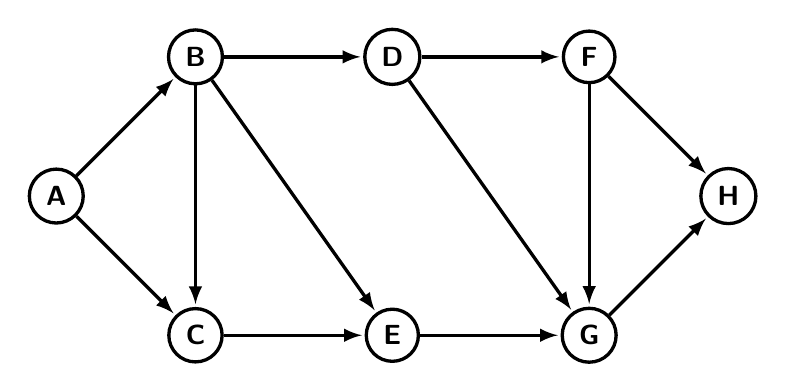
\begin{tikzpicture} [node distance = 2.5cm, very thick, main/.style = {draw, circle, font=\sffamily\bfseries}, edge/.style={->,> = latex, shorten > = 1pt}]
			\node[main] (B) {B};
                \node[main, below left of = B] (A) {A};
			\node[main, below  right of = A] (C) {C};
			\foreach \i\j in {B/D, D/F, C/E, E/G} {
					\node[main, circle, right of = \i] (\j) {\j};
				}
                \node[main, below right of = F] (H) {H};
			\draw[edge] (A) -- (B);
			\foreach \i\j in {B/C, A/C, B/D, D/F, C/E, E/G, B/E, D/G, F/H, G/H} {
					\draw[edge] (\i) -- (\j);
				}
			\draw[edge] (F) -- (G);
		\end{tikzpicture}
	\end{center}
	\begin{choices}
    	\choice 	    A B C E G D F H
		\choice 	A B C D E F G H
		\choice 	A B D C F E G H
		\choice 	    A B D E C F G H
	\end{choices}

\part[2]For the coin-changing problem, denote
    \begin{itemize}
        \item $C=(c_1, c_2,\cdots,c_k)$: the denominations of coins, where $1=c_1<c_2<\dots<c_k$;
        \item $X_n^*$: an optimal solution, i.e., a multi-set of coins which has the minimum number of coins to make change for $n$;
        \item $X_n$: the greedy solution, solved by
        \[
        X_n=\begin{cases}
        \{ \},&n=0\\
        \{c_t\}\cup X_{n-c_t},&n\ge 1, \text{where } c_t=\max\limits_{c_i\le n}c_i \text{ is the largest coin that can be used}
        \end{cases}
        \]
    \end{itemize}

For example, if $C=(1,2,3)$, then $X_4^*$ can be either $\{2,2\}$ or $\{3,1\}$, and $X_4=\{3,1\}$.

Which of the following statements is/are true?

    \begin{choices}
 
        \choice If $\forall i\in[3,n], c_i=c_{i-1}+c_{i-2}$, then $\forall n,|X_n^*|=|X_n|$.
        \choice $\exists C,\exists i$ with $2c_i>c_{i+1}$, such that $\forall n,|X_n^*|=|X_n|$.
        \choice If $\forall i, 2c_i\le c_{i+1}$, then $\forall n,|X_n^*|=|X_n|$.
        \choice If $\forall i\in[2,n], \dfrac{c_i}{c_{i-1}}$ is an integer, then $\forall n,|X_n^*|=|X_n|$.
 
    \end{choices}

\end{parts} 

\newpage
